\documentclass{standalone}
\usepackage{tikz}
\usepackage{amsmath}
\usetikzlibrary{decorations.pathmorphing}

\begin{document}
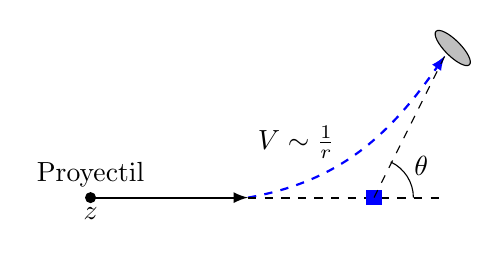
\begin{tikzpicture}

    \fill[] (-2,1) circle (2pt) node[black,yshift=-0.2cm] {$z$};
    % Escala
    
    \draw[thick,-latex] (-2,1) node[above]{Proyectil}-- (0,1);


    \draw[thick, blue, dashed, -latex] (0,1) to[out=10, in=235](2.5,2.8);

    \draw[thick, dashed] (0,1)--(2.5,1);

    \fill[blue] (1.7,1.1) rectangle (1.5,0.9);
    \draw[dashed] (1.6,1)--(2.5,2.8);
    
    \node[right] at(0,1.7){$V\sim \frac{1}{r}$};

    \draw[rotate around={-45:(2.6,2.9)}, fill=lightgray] (2.6,2.9)ellipse (0.3 and 0.1);
    
     \draw (2.1,1) arc[start angle=0, end angle=65, radius=0.5];
     \node at(2.2,1.4){$\theta$};
\end{tikzpicture}
\end{document}